%%% Hlavní soubor. Zde se definují základní parametry~a odkazuje se na ostatní části. %%%

%% Verze pro jednostranný tisk:
% Okraje: levý 40mm, pravý 25mm, horní~a dolní 25mm
% (ale pozor, LaTeX si sám přidává 1in)
\documentclass[12pt,a4paper]{report}
\setlength\textwidth{145mm}
\setlength\textheight{247mm}
\setlength\oddsidemargin{15mm}
\setlength\evensidemargin{15mm}
\setlength\topmargin{0mm}
\setlength\headsep{0mm}
\setlength\headheight{0mm}
% \openright zařídí, aby následující text začínal na pravé straně knihy
\let\openright=\clearpage

%% Pokud tiskneme oboustranně:
% \documentclass[12pt,a4paper,twoside,openright]{report}
% \setlength\textwidth{145mm}
% \setlength\textheight{247mm}
% \setlength\oddsidemargin{14.2mm}
% \setlength\evensidemargin{0mm}
% \setlength\topmargin{0mm}
% \setlength\headsep{0mm}
% \setlength\headheight{0mm}
% \let\openright=\cleardoublepage

\usepackage[colorlinks=false,urlcolor=black,bookmarksopen=true]{hyperref} 	% Záložky v souboru

%% Vytváříme PDF/A-2u
\usepackage[a-2u]{pdfx}

%% Přepneme na českou sazbu~a fonty Latin Modern
\usepackage[czech]{babel}
\usepackage{lmodern}
\usepackage[T1]{fontenc}
\usepackage{textcomp}

%% Použité kódování znaků: obvykle latin2, cp1250~nebo utf8:
\usepackage[utf8]{inputenc}
\usepackage{csquotes}
\MakeOuterQuote{"}

%%% Další užitečné balíčky (jsou součástí běžných distribucí LaTeXu)
\usepackage{amsmath}        % rozšíření pro sazbu matematiky
\usepackage{amsfonts}       % matematické fonty
\usepackage{amsthm}         % sazba vět, definic apod.
\usepackage{amssymb}
\usepackage{bbding}         % balíček s nejrůznějšími symboly
			    % (čtverečky, hvězdičky, tužtičky, nůžtičky, ...)
\usepackage{bm}             % tučné symboly (příkaz \bm)
\usepackage{graphicx}       % vkládání obrázků
\usepackage{fancyvrb}       % vylepšené prostředí pro strojové písmo
\usepackage{indentfirst}    % zavede odsazení 1. odstavce kapitoly
\usepackage[numbers]{natbib}         % zajištuje možnost odkazovat na literaturu
			    % stylem AUTOR (ROK), resp. AUTOR [ČÍSLO]
\usepackage[nottoc]{tocbibind} % zajistí přidání seznamu literatury,
                            % obrázků~a tabulek do obsahu
\usepackage{icomma}         % inteligetní čárka v matematickém módu
\usepackage{dcolumn}        % lepší zarovnání sloupců v tabulkách
\usepackage{booktabs}       % lepší vodorovné linky v tabulkách
\usepackage{paralist}       % lepší enumerate~a itemize
\usepackage{xcolor}         % barevná sazba
\usepackage{float}
\usepackage{ifthen}
\usepackage{cancel}
\usepackage{enumitem}
\usepackage{ragged2e}
\usepackage{needspace}
\usepackage{pgfplots}
\usepackage{subcaption}
\pgfplotsset{compat=1.15}
\usepackage{mathrsfs}
\usetikzlibrary{arrows}

\justifying

\graphicspath{{./components/images/}}

%%% Údaje o~práci

% Název práce v~jazyce práce (přesně podle zadání)
\def\NazevPrace{Stručný úvod do teorie množin pro středoškoláky}

% Název práce v~angličtině
\def\NazevPraceEN{A Brief Introduction to Set Theory for High Schools}

% Jméno autora
\def\AutorPrace{David Weber}

% Rok odevzdání
\def\RokOdevzdani{2022}

% Název katedry nebo ústavu, kde byla práce oficiálně zadána
% (dle Organizační struktury MFF UK, případně plný název pracoviště mimo MFF)
\def\Katedra{Katedra didaktiky matematiky}
\def\KatedraEN{Department of Mathematics Education}

% Jedná se o~katedru (department) nebo o~ústav (institute)?
\def\TypPracoviste{Katedra}
\def\TypPracovisteEN{Department}

% Vedoucí práce: Jméno a~příjmení s~tituly
\def\Vedouci{RNDr.~Martin~Rmoutil,~Ph.D.}

% Pracoviště vedoucího (opět dle Organizační struktury MFF)
\def\KatedraVedouciho{Katedra didaktiky matematiky}
\def\KatedraVedoucihoEN{Department of Mathematics Education}

% Studijní program a~obor
\def\StudijniProgram{Matematika se zaměřením na vzdělávání}
\def\StudijniObor{Matematika se zaměřením na vzdělávání se sdruženým studiem informatika se zaměřením na vzdělávání}

% Nepovinné poděkování (vedoucímu práce, konzultantovi, tomu, kdo
% zapůjčil software, literaturu apod.)
\def\Podekovani{%
Zde bych rád poděkoval RNDr. Martinu Rmoutilovi, Ph.D. za jeho vstřícný přístup, cenné rady a~množství času, které mi věnoval v~době psaní této bakalářské práce. Dále patří velké poděkování Michaele Dvořákové za pomoc při korekci gramatiky a~pravopisu a~Martinu Kopeckému za poskytnutí grafické ilustrace domina v~příloze. Též chci poděkovat své rodině za trpělivost a~pomoc při psaní této práce.
}

% Abstrakt (doporučený rozsah cca 80-200 slov; nejedná se o~zadání práce)
\def\Abstrakt{%
%%% Šablona pro jednoduchý soubor formátu PDF/A, jako třeba samostatný abstrakt práce.

\documentclass[12pt]{report}

\usepackage[a4paper, hmargin=1in, vmargin=1in]{geometry}
\usepackage[a-2u]{pdfx}
\usepackage[czech]{babel}
\usepackage[utf8]{inputenc}
\usepackage{csquotes}
\MakeOuterQuote{"}
\usepackage[T1]{fontenc}
\usepackage{lmodern}
\usepackage{textcomp}

\begin{document}

%% Nezapomeňte upravit abstrakt.xmpdata.

\noindent\textbf{Abstrakt:}\quad%%% Šablona pro jednoduchý soubor formátu PDF/A, jako třeba samostatný abstrakt práce.

\documentclass[12pt]{report}

\usepackage[a4paper, hmargin=1in, vmargin=1in]{geometry}
\usepackage[a-2u]{pdfx}
\usepackage[czech]{babel}
\usepackage[utf8]{inputenc}
\usepackage{csquotes}
\MakeOuterQuote{"}
\usepackage[T1]{fontenc}
\usepackage{lmodern}
\usepackage{textcomp}

\begin{document}

%% Nezapomeňte upravit abstrakt.xmpdata.

\noindent\textbf{Abstrakt:}\quad%%% Šablona pro jednoduchý soubor formátu PDF/A, jako třeba samostatný abstrakt práce.

\documentclass[12pt]{report}

\usepackage[a4paper, hmargin=1in, vmargin=1in]{geometry}
\usepackage[a-2u]{pdfx}
\usepackage[czech]{babel}
\usepackage[utf8]{inputenc}
\usepackage{csquotes}
\MakeOuterQuote{"}
\usepackage[T1]{fontenc}
\usepackage{lmodern}
\usepackage{textcomp}

\begin{document}

%% Nezapomeňte upravit abstrakt.xmpdata.

\noindent\textbf{Abstrakt:}\quad\input{abstract.txt}

\end{document}


\end{document}


\end{document}

}
\def\AbstraktEN{%
%%% Šablona pro jednoduchý soubor formátu PDF/A, jako třeba samostatný abstrakt práce.

\documentclass[12pt]{report}

\usepackage[a4paper, hmargin=1in, vmargin=1in]{geometry}
\usepackage[a-2u]{pdfx}
\usepackage[english]{babel}
\usepackage[utf8]{inputenc}
\usepackage[T1]{fontenc}
\usepackage{lmodern}
\usepackage{textcomp}

\begin{document}

%% Nezapomeňte upravit abstrakt.xmpdata.

\noindent\textbf{Abstract:}\quad%%% Šablona pro jednoduchý soubor formátu PDF/A, jako třeba samostatný abstrakt práce.

\documentclass[12pt]{report}

\usepackage[a4paper, hmargin=1in, vmargin=1in]{geometry}
\usepackage[a-2u]{pdfx}
\usepackage[english]{babel}
\usepackage[utf8]{inputenc}
\usepackage[T1]{fontenc}
\usepackage{lmodern}
\usepackage{textcomp}

\begin{document}

%% Nezapomeňte upravit abstrakt.xmpdata.

\noindent\textbf{Abstract:}\quad%%% Šablona pro jednoduchý soubor formátu PDF/A, jako třeba samostatný abstrakt práce.

\documentclass[12pt]{report}

\usepackage[a4paper, hmargin=1in, vmargin=1in]{geometry}
\usepackage[a-2u]{pdfx}
\usepackage[english]{babel}
\usepackage[utf8]{inputenc}
\usepackage[T1]{fontenc}
\usepackage{lmodern}
\usepackage{textcomp}

\begin{document}

%% Nezapomeňte upravit abstrakt.xmpdata.

\noindent\textbf{Abstract:}\quad\input{abstract_en.txt}

\end{document}

\end{document}

\end{document}
}

% 3 až 5 klíčových slov (doporučeno), každé uzavřeno ve složených závorkách
\def\KlicovaSlova{%
{teorie množin}, {kardinál}, {ordinál}, {přirozené číslo}, {nekonečno}, {Georg Cantor}, {Bernard Bolzano}
}
\def\KlicovaSlovaEN{%
{set theory}, {cardinal number}, {ordinal number}, {natural number}, {infinity}, {Georg Cantor}, {Bernard Bolzano}
}

%% Balíček hyperref, kterým jdou vyrábět klikací odkazy v~PDF,
%% ale hlavně ho používáme k~uložení metadat do PDF (včetně obsahu).
%% Většinu nastavítek přednastaví balíček pdfx.
\hypersetup{unicode}
\hypersetup{breaklinks=true}

%% Definice různých užitečných maker (viz popis uvnitř souboru)
%%% Tento soubor obsahuje definice různých užitečných maker a prostředí %%%
%%% Další makra připisujte sem, ať nepřekáží v ostatních souborech.     %%%

%%% Drobné úpravy stylu

% Tato makra přesvědčují mírně ošklivým trikem LaTeX, aby hlavičky kapitol
% sázel příčetněji a nevynechával nad nimi spoustu místa. Směle ignorujte.
%\makeatletter
%\def\@makechapterhead#1{
%  {\parindent \z@ \raggedright \normalfont
%   \Huge\bfseries \thechapter. #1
%   \par\nobreak
%   \vskip 20\p@
%}}
%\def\@makeschapterhead#1{
%  {\parindent \z@ \raggedright \normalfont
%   \Huge\bfseries #1
%   \par\nobreak
%   \vskip 20\p@
%}}
%\makeatother

\setlength{\parskip}{0.3em}

% Toto makro definuje kapitolu, která není očíslovaná, ale je uvedena v obsahu.
\def\chapwithtoc#1{
\chapter*{#1}
\addcontentsline{toc}{chapter}{#1}
}

% Trochu volnější nastavení dělení slov, než je default.
\lefthyphenmin=2
\righthyphenmin=2

% Zapne černé "slimáky" na koncích řádků, které přetekly, abychom si
% jich lépe všimli.
\overfullrule=1mm

%%% Makra pro definice, věty, tvrzení, příklady, ... (vyžaduje baliček amsthm)

\theoremstyle{plain}
\newtheorem{theorem}{Věta}[section]
\newtheorem{lemma}[theorem]{Lemma}
\newtheorem{proposition}[theorem]{Tvrzení}
\newtheorem{corollary}[theorem]{Důsledek}
\newtheorem*{proposition*}{Tvrzení}

\theoremstyle{definition}
\newtheorem{definition}[theorem]{Definice}
\newtheorem{example}[theorem]{Příklad}
\newtheorem{remark}[theorem]{Poznámka}
\newtheorem{convention}[theorem]{Úmluva}
\newtheorem{denoting}[theorem]{Značení}

%%% Prostředí pro důkazy

\renewenvironment{proof}[1][]{
  \par\medskip\noindent
  \textit{\ifthenelse{\equal{#1}{}}
  {Důkaz}
  {#1}}.
}{
\hspace*{\fill}$\qedsymbol$\par\medskip
}
\newenvironment{solution}{
  \par\medskip\noindent
  \textit{Řešení}.
}{
\hspace*{\fill}$\qedsymbol$\par\medskip
}

%%% Prostředí pro sazbu kódu, případně vstupu/výstupu počítačových
%%% programů. (Vyžaduje balíček fancyvrb -- fancy verbatim.)

\DefineVerbatimEnvironment{code}{Verbatim}{fontsize=\small, frame=single}

%%% Prostor reálných čísel, přirozených čísel, ...
\newcommand{\R}{\mathbb{R}}
\newcommand{\C}{\mathbb{C}}
\newcommand{\N}{\mathbb{N}}
\newcommand{\Q}{\mathbb{Q}}
\newcommand{\Z}{\mathbb{Z}}

%%% Užitečné operátory pro statistiku a pravděpodobnost
\DeclareMathOperator{\pr}{\textsf{P}}
\DeclareMathOperator{\E}{\textsf{E}\,}
\DeclareMathOperator{\var}{\textrm{var}}
\DeclareMathOperator{\sd}{\textrm{sd}}
\DeclareMathOperator{\arctg}{arctg}
\DeclareMathOperator{\tg}{tg}

%%% Příkaz pro transpozici vektoru/matice
\newcommand{\T}[1]{#1^\top}

%%% Vychytávky pro matematiku
\newcommand{\goto}{\rightarrow}
\newcommand{\gotop}{\stackrel{P}{\longrightarrow}}
\newcommand{\maon}[1]{o(n^{#1})}
\newcommand{\abs}[1]{\left|{#1}\right|}
\newcommand{\dint}{\int_0^\tau\!\!\int_0^\tau}
\newcommand{\isqr}[1]{\frac{1}{\sqrt{#1}}}

\newcommand{\napprox}{\not\approx}
\newcommand{\norm}[1]{|| #1 ||}
\newcommand{\dotprod}[2]{\left(#1|#2\right)}
\newcommand{\compl}[1]{#1^\complement}
\newcommand{\map}[3]{#1:#2 \rightarrow #3}
\newcommand{\mapto}[3]{#1:#2 \mapsto #3}
\newcommand{\powset}[1]{\mathcal{P}\left(#1\right)}
\newcommand{\solutions}[1]{\left[K=\left\{#1\right\}\right]}
\newcommand{\set}[1]{\left\{#1\right\}}
\newcommand{\admid}{\;\middle\vert\;}
\newcommand{\sizeof}[1]{\left|#1\right|}
\newcommand{\dx}[1][]{
   \ifthenelse{\equal{#1}{}}%
      {\ensuremath{\,\mathrm{d}x}}%
      {\ensuremath{\,\mathrm{d}#1}}%
} % diferenciál

\newcommand{\ZF}{\textsf{ZF}} % Zermelova-Fraenkelova teorie množin
\newcommand{\PA}{\textsf{PA}} % Peanova aritmetika

% Čítače
\newcommand{\createcnt}[2][0]{\newcounter{#2}\setcounter{#2}{#1}}
\newcommand{\printcnt}[1]{\arabic{#1}}
\newcommand{\printnstepcnt}[1]{\stepcounter{#1}\arabic{#1}}

%%% Vychytávky pro tabulky
\newcommand{\pulrad}[1]{\raisebox{1.5ex}[0pt]{#1}}
\newcommand{\mc}[1]{\multicolumn{1}{c}{#1}}

% Full Names
\newcommand{\name}[1]{\mbox{\textsc{#1}}}

% Logical operators
\renewcommand{\implies}{\Rightarrow}
\renewcommand{\impliedby}{\Leftarrow}
\renewcommand{\iff}{\Leftrightarrow}

% Paths
\newcommand{\chapterpath}[1]{components/ch#1}
\newcommand{\sectionpath}[1]{components/ch#1/sections}
\newcommand{\literaturepath}{components/literature}
\newcommand{\appendixpath}{components/appendix}

% TODO
\newcommand{\todo}[1]{\textcolor{red}{(\noindent TODO: #1.)}}

% Rightsided note
\newcommand{\rightnote}[1]{\hspace*{\fill} $\triangleleft$ \textit{#1}}

% Images
\newcommand{\fullhd}{0.2}
\newcommand{\normalipe}{0.8}

%% Titulní strana a~různé povinné informační strany
\begin{document}
%%% Titulní strana práce a další povinné informační strany

%%% Titulní strana práce

\pagestyle{empty}
\hypersetup{pageanchor=false}

\begin{center}

\centerline{\mbox{
\includegraphics[width=166mm]{components/images/logo-cs.pdf}}}

\vspace{-8mm}
\vfill

{\bf\Large BAKALÁŘSKÁ PRÁCE}

\vfill

{\LARGE\AutorPrace}

\vspace{15mm}

{\LARGE\bfseries\NazevPrace}

\vfill

\Katedra

\vfill

{
\centerline{\vbox{\halign{\hbox to 0.45\hsize{\hfil #}&\hskip 0.5em\parbox[t]{0.45\hsize}{\raggedright #}\cr
Vedoucí bakalářské práce:&\Vedouci \cr
\noalign{\vspace{2mm}}
Studijní program:&\StudijniProgram \cr
\noalign{\vspace{2mm}}
Studijní obor:&\StudijniObor \cr
}}}}

\vfill

% Zde doplňte rok
Praha \RokOdevzdani

\end{center}

\newpage

%%% Následuje vevázaný list -- kopie podepsaného "Zadání bakalářské práce".
%%% Toto zadání NENÍ součástí elektronické verze práce, nescanovat.

%%% Strana s čestným prohlášením k~bakalářské práci

\openright
\hypersetup{pageanchor=true}
\pagestyle{plain}
\pagenumbering{roman}
\vglue 0pt plus 1fill

\noindent
Prohlašuji, že jsem tuto bakalářskou práci vypracoval(a) samostatně a výhradně
s~použitím citovaných pramenů, literatury a dalších odborných zdrojů.
Tato práce nebyla využita k~získání jiného nebo stejného titulu.

\medskip\noindent
Beru na~vědomí, že se na moji práci vztahují práva a povinnosti vyplývající
ze zákona č. 121/2000 Sb., autorského zákona v~platném znění, zejména skutečnost,
že Univerzita Karlova má právo na~uzavření licenční smlouvy o~užití této
práce jako školního díla podle §60 odst. 1 autorského zákona.

\vspace{10mm}

\hbox{\hbox to 0.5\hsize{%
V \hbox to 6em{\dotfill} dne \hbox to 6em{\dotfill}
\hss}\hbox to 0.5\hsize{\dotfill\quad}}
\smallskip
\hbox{\hbox to 0.5\hsize{}\hbox to 0.5\hsize{\hfil Podpis autora\hfil}}

\vspace{20mm}
\newpage

%%% Poděkování

\openright

\noindent
\Podekovani

\newpage

%%% Povinná informační strana bakalářské práce

\openright

\vbox to 0.5\vsize{
\setlength\parindent{0mm}
\setlength\parskip{5mm}

Název práce:
\NazevPrace

Autor:
\AutorPrace

\TypPracoviste:
\Katedra

Vedoucí bakalářské práce:
\Vedouci, \KatedraVedouciho

Abstrakt:
\Abstrakt

Klíčová slova:
\KlicovaSlova

\vss}

\newpage

\nobreak\vbox to 0.49\vsize{
\setlength\parindent{0mm}
\setlength\parskip{5mm}

Title:
\NazevPraceEN

Author:
\AutorPrace

\TypPracovisteEN:
\KatedraEN

Supervisor:
\Vedouci, \KatedraVedoucihoEN

Abstract:
\AbstraktEN

Keywords:
\KlicovaSlovaEN

\vss}

\newpage

\openright
\pagestyle{plain}
\pagenumbering{arabic}
\setcounter{page}{1}


%%% Strana s automaticky generovaným obsahem bakalářské práce

\tableofcontents

%%% Obrázky v~bakalářské práci
%%% (pokud jich je malé množství, obvykle není třeba seznam uvádět)
\listoffigures

%%% Jednotlivé kapitoly práce jsou pro přehlednost uloženy v~samostatných souborech

\include{\chapterpath{01}/historie_tm.tex}
\include{\chapterpath{02}/logika.tex}
\include{\chapterpath{03}/axiomy_tm.tex}
\include{\chapterpath{04}/relace.tex}
\include{\chapterpath{05}/budovani_ciselnych_mnozin.tex}
\include{\chapterpath{06}/porovnavani_nekonecnych_mnozin.tex}

%%% Seznam použité literatury
%%% Seznam použité literatury (bibliografie)
%%%
%%% Pro vytváření bibliografie používáme bibTeX. Ten zpracovává
%%% citace v textu (např. makro \cite{...}) a vyhledává k nim literaturu
%%% v souboru literatura.bib.
%%%
%%% Příkaz \bibliographystyle určuje, jakým stylem budou citovány odkazy
%%% v textu. V závorce je název zvoleného souboru .bst. Styly plainnat
%%% a unsrt jsou standardní součástí latexových distribucí. Styl czplainnat
%%% je dodáván s touto šablonou a bibTeX ho hledá v aktuálním adresáři.

% \bibliographystyle{czplainnat}    %% Autor (rok) s českými spojkami
% \bibliographystyle{plainnat}    %% Autor (rok) s anglickými spojkami
\bibliographystyle{unsrtnat}       %% [číslo]

\renewcommand{\bibname}{Seznam použité literatury}

%%% Vytvoření seznamu literatury. Pozor, pokud jste necitovali ani jednu
%%% položku, seznam se automaticky vynechá.

\bibliography{\literaturepath/literature.bib}

%%% Kdybyste chtěli bibliografii vytvářet ručně (bez bibTeXu), lze to udělat
%%% následovně. V takovém případě se řiďte normou ISO 690 a zvyklostmi v oboru.

% \begin{thebibliography}{99}
%
% \bibitem{lamport94}
%   {\sc Lamport,} Leslie.
%   \emph{\LaTeX: A Document Preparation System}.
%   2. vydání.
%   Massachusetts: Addison Wesley, 1994.
%   ISBN 0-201-52983-1.
%
% \end{thebibliography}


%%% Tabulky v~bakalářské práci (opět nemusí být nutné uvádět)
%%% U matematických prací může být lepší přemístit seznam tabulek na začátek práce.
% \listoftables

%%% Přílohy k~bakalářské práci, existují-li. Každá příloha musí být alespoň jednou
%%% odkazována z vlastního textu práce. Přílohy se číslují.
%%%
%%% Do tištěné verze se spíše hodí přílohy, které lze číst a~prohlížet (dodatečné
%%% tabulky a~grafy, různé textové doplňky, ukázky výstupů z počítačových programů,
%%% apod.). Do elektronické verze se hodí přílohy, které budou spíše používány
%%% v~elektronické podobě než čteny (zdrojové kódy programů, datové soubory,
%%% interaktivní grafy apod.). Elektronické přílohy se nahrávají do SISu a~lze
%%% je také do práce vložit na CD/DVD. Povolené formáty souborů specifikuje
%%% opatření rektora č. 72/2017.

\appendix
\chapter{Důkazy}\label{chap:dukazy}
V~matematice se lze setkat s~celou řadou různých tvrzení. Od primitivních, jejichž platnost je zřejmá až po složitější, nad jejich platností je třeba se více zamyslet. Čtenář se nejspíše zatím spíše setkával s~matematikou, která zahrnovala užívání jistých postupů. Např. zjednodušování algebraických výrazů, řešení soustav rovnic, ověřování trigonometrických identit, aj. Avšak hodně postupe v~tatematice je založeno na již známých výsledcích, o~nichž bylo dokázáno, že jsou pravdivé. Pokud ovšem máme dokázat určité tvrzení, je třeba, aby bylo naše zdůvodnění jednoznačné a logicky správné. V~této sekci se proto podíváme na důkazové techniky používane v~tatematice, které budeme dále v~textu využívat.\par
Matematická tvrzení jsou často různě klasifikována v~závislosti na jejich povaze. Základními typy jsou tyto. 
\begin{itemize}
    \item \emph{Axiom}. Tvrzení, které implicitně považujeme za pravdivé a nedokazujeme jej. S~axiomatikou jsme se již částečně seznámili v~historické předmluvě (viz \ref{subsec:tm_soucasnost}).
    \item \emph{Věta}. Matematické tvrzení, jehož pravdivost můžeme ověřit důkazem.
    \item \emph{Lemma}. Pomocné tvrzení, které běžně využíváme pro důkaz jiného (typicky složitějšího) tvrzení.
    \item \emph{Důsledek}. Tvrzení, které je přímým důsledkem jiného tvrzení.
\end{itemize}
Čistě formálně však mezi \textbf{větou}, \textbf{lemmatem} a \textbf{důsledkem} není žádný rozdíl.

\section{Důkaz přímý}\label{sec:dukaz_primy}
Jedná se o~asi nejjednodušší typ důkazu. Často jsou matematická tvrzení formulována jako implikace, tzn. "Jestliže platí $A$, pak platí $B$.". Konkrétně, např. "Je-li $x<0$, pak $x^2>0$.".\par
Myšlenka důkazu je taková, že začínáme od předpokladu $A$, z~něhož dále odvozujeme dílčí tvrzení tak dlouho, až dojdeme k~požadovanému závěru $B$. Symbolicky, pokud si označíme dílčí tvrzení v~důkazu $X_1, X_2, \dots, X_n$, pak vlastně dokazujeme výrokovou formuli
\begin{equation}\label{eq:primy_dukaz_formule}
    (A~\implies X_1) \land (X_1 \implies X_2) \land \cdots \land (X_{n-1}\implies X_n) \land (X_n \implies B).
\end{equation}
V~tomto procesu dokazování se využívá tautologie \ref{item:tautologie_4} z~věty \ref{thm:vyznamne_tautologie}
\begin{equation*}
    (A~\implies B) \land (B \implies C) \iff (A~\implies C).
\end{equation*}
Z~tohoto faktu vyplývá, že pokud je každá z~dílčích implikací pravdivá, pak je nutně pravdivá i implikace $A \implies B$, kterou jsme chtěli dokázat\footnote{Výrokové proměnné lze v~konkrétním případě nahradit příslušnými predikáty.}. Podívejme se na příklad podobný příklad z~úvodu.

\begin{proposition}
    Nechť $x\in\R$. Je-li $x<0$, pak $x^2+1>0$.
\end{proposition}
\begin{proof}
    Předpokladem našeho tvrzení je $x\in\R \land x<0$. Víme, že pro každé reálné číslo $x$ platí, že $x^2\geq 0$. Tj. určitě platí implikace
    \begin{equation*}
        x<0 \implies x^2>0.
    \end{equation*}
    Dále víme, že triviálně platí $1>0$, tedy také jistě platí
    \begin{equation*}
        x^2+1>x^2.
    \end{equation*}
    Protože však $x^2>0$, pak také
    $x^2+1>0$, což jsme chtěli dokázat.
\end{proof}
Posloupnost dokázaných implikací bychom mohli podle \eqref{eq:primy_dukaz_formule} zapsat nyní jako
\begin{equation*}
    (x\in\R \land x<0 \implies x^2>0) \land (x^2>0 \implies x^2+1>x^2) \land (x^2+1>x^2 \implies x^2+1>0),
\end{equation*}
a tedy jsme dokázali i implikaci v~původním tvrzení $x<0 \implies x^2+1>0$.\par
V~praxi důkazy takto samozřejmě nerozepisujeme a řadu věcí považujeme za samozřejmé, např. právě $1>0$, $x^2+1>x^2$, apod. Takový důkaz bychom bez většího rozepisování mohli napsat klidně na jeden řádek.
\begin{equation*}
    x<0 \implies 0<x^2<x^2+1 \implies x^2+1>0.
\end{equation*}
Všimněte si zároveň, že jsme zde použili jistou generalizaci. Předvedený důkaz totiž není závislý na volbě $x$ a náš argument je tak univerzální. Tedy platí
\begin{equation*}
    \forall x<0: x^2+1>0.
\end{equation*}
Obecně tvrzení formulovaná stylem "je-li $x\in X$, pak \dots" jsou míněna jako
\begin{equation*}
    \forall x\in X: \dots
\end{equation*}
\begin{proposition}
    Nechť $n\in\N$ je liché. Pak $3n+7$ je sudé číslo.
\end{proposition}
\begin{proof}
    Začneme u~předpokladu, že $n\in\N$ je liché číslo. To znamená, že
    \begin{equation*}
        \exists k\in\N : n=2k+1.
    \end{equation*}
    Po dosazení obdržíme
    \begin{equation*}
        3(2k+1)+7=6k+3+7=6k+10=2(3k+5).
    \end{equation*}
    Protože $3k+5$ je přirozené číslo, pak $3n+7$ je dělitelné dvěma a je tedy sudé, což jsme chtěli dokázat.
\end{proof}
\begin{proposition}[AG nerovnost]
    Pro $a,b\in\R_0^+$ platí
    \begin{equation*}
        \sqrt{ab}\leq\dfrac{a+b}{2}.
    \end{equation*}
\end{proposition}
\begin{proof}
    Při důkazu tohoto tvrzení vyjdeme z~jednoduchého pozorování:
    \begin{equation*}
        (\sqrt{a}+\sqrt{b})^2\geq 0.
    \end{equation*}
    Nyní stačí výraz upravit a dostaneme požadovanou nerovnost.
    \begin{equation*}
        (\sqrt{a}+\sqrt{b})^2 = a+2\sqrt{ab}+b\geq 0 \implies \sqrt{ab}\leq \dfrac{a+b}{2}.
    \end{equation*}
\end{proof}
\begin{proposition}
    Pro $\forall x,y\in\R$ platí
    \begin{equation*}
        x<y \implies x<\dfrac{x+y}{2}<y.
    \end{equation*}
\end{proposition}
\begin{proof}
    Zde je třeba si všimnout "dvojité" nerovnosti v~dokazovaném tvrzení. To nám již napovídá, že ve skutečnosti musíme dokázat 2 dílčí tvrzení, konkrétně
    \begin{equation*}
        x < \dfrac{x+y}{2}\quad\text{a}\quad\dfrac{x+y}{2} < y.
    \end{equation*}
    Při důkazu obou částí vyjdeme opět z~předpokladu. Tedy mějme libovolná čísla $x,y\in\R$ taková, že $x<y$. Pak jistě platí
    \begin{equation*}
        x+x<x+y \implies 2x<x+y \implies x<\dfrac{x+y}{2}.
    \end{equation*}
    Tím jsme dokázali první nerovnost. Platnost druhé dokážeme analogicky:
    \begin{equation*}
        x+y<y+y \implies x+y<2y \implies \dfrac{x+y}{2}<y.
    \end{equation*}
\end{proof}
(Převzato z~\cite{ChartrandPolimeniZhang2014}, str. 79 a \cite{MatematickaLogikaUK2010}, sekce \emph{důkaz přímý}.)\\
Ne všechna tvrzení jsou v~matematice nutně formulována jako implikace. Často se lze setkat s~tvrzeními formulovanými jako ekvivalence, tj. $A \iff B$. Důkazy takových výroků jsou již trochu delší, neboť už nestačí pouze ukázat $A \implies B$. Vzpomeňme si však na tautologii, která nám dávala do souvislosti ekvivalenci s~implikací (viz \ref{item:tautologie_2} ve větě \ref{thm:vyznamne_tautologie}):
\begin{equation*}
    (A~\iff B) \iff (A~\implies B) \land (B \implies A).
\end{equation*}
Z~toho je již vidět, jak u~takových tvrzení při důkazu postupovat. Zkrátka dokážeme zvlášť $A \implies B$ a $A \impliedby B$.
\begin{proposition}
    Nechť $x,y\in\Z$. Pak $3 \mid xy$ právě tehdy, když $3 \mid x$ nebo $3 \mid y$.
\end{proposition}
\begin{proof}
    \textit{($\implies$)}. Začneme s~předpokladem, že $3 \mid xy$. Víme, že pokud je číslo dělitelné třemi, pak jej lze zapsat jako $3k$, kde $k\in\Z$. Uvažujme následující případy:
    \begin{itemize}
        \item $3 \mid x \land 3 \mid y$. Tehdy tvrzení jistě platí.
        \item $3 \nmid x$. Ukážeme, že pak nutně musí platit $3 \mid y$. Pokud $x$ není dělitelné třemi, pak jej lze zapsat buď jako $3k+1$, nebo $3k+2$, kde $k\in\Z$. 
        \begin{equation*}
            xy=(3k+1)y\quad\text{nebo}\quad xy=(3k+2)y
        \end{equation*}
        Protože čísla $3k+1$ a $3k+2$ nejsou dělitelná třemi, pak je vidět, že musí platit $3 \mid y$.
        \item $3 \nmid y$. Zde je postup analogický. 
    \end{itemize}
    Tím máme dokázanou implikaci $3 \mid xy \implies 3 \mid x \lor 3 \mid y$.\\
    \textit{($\impliedby$)}. Nyní předpokládáme, že platí $3 \mid x \lor 3 \mid y$; chceme ukázat, že $3 \mid xy$ Bez újmy na obecnosti\footnote{Termín \emph{bez újmy na obecnosti} (někdy zkráceně \emph{BÚNO}) se v~matematických textech používe v~mituacích, kdy může nastat více možností, avšak říkáme, že jejich důkazy jsou analogické.}, nechť je $x$ dělitelné třemi. Pak existuje $x=3k$, kde $k\in\Z$. Po dosazení dostaneme
    \begin{equation*}
        xy=(3k)y=3(ky) \implies 3 \mid xy.
    \end{equation*}
    Tedy dokázali jsme obě implikace a tím i původní tvrzení.
\end{proof}

\section{Důkaz nepřímý}\label{sec:dukaz_neprimy}
Řada tvrzení v~matematice však není až tak jednoduchá na dokázání přímo. Důkazy, které jsme si ukazovali, vždy začínaly od předpokladu a postupně jsme došli k~požadovanému závěru. Lze ale postupovat i jinak. Opět se odkážeme na dříve zmíněné tautologie věty \ref{thm:vyznamne_tautologie}, konkrétně na \ref{item:tautologie_5}:
\begin{equation}\label{eq:dukaz_neprimy_tautologie}
    (A~\implies B) \iff (\neg B \implies \neg A).
\end{equation}
Implikace je ve skutečnosti ekvivalentní s~tvrzením, že pokud neplatí závěr, pak neplatí ani předpoklad. Na této skutečnosti je založen \emph{důkaz nepřímý} (též \emph{důkaz obměnou}). Podívejme se na příklady užití.
\begin{proposition}
    Nechť $x\in\Z$ a $3 \nmid (x^2-1)$. Pak $3 \mid x$.
\end{proposition}
V~tomto případě máme dvě možnosti. Buď začneme s~předpokladem $3 \nmid (x^2-1)$ a dokážeme, že $3 \mid x$ (tedy dokážeme tvrzení přímo), nebo naopak budeme předpokládat, že $3 \nmid x$ a dokážeme negaci původního předpokladu. Ačkoliv by se jistě našla možnost, jak tvrzení dokázat přímo, přesto se nejspíše zdá jednodušší začít s~předpokladem, že $x$ není dělitelné třemi.
\begin{proof}
    Nechť $3 \nmid x$. Ukážeme, že platí $3 \mid (x^2-1)$. Podle předpokladu lze $x$ zapsat jako $3k+1$ nebo $3k+2$, kde $k\in\Z$. Bez újmy na obecnosti pišme $x=3k+1$. Pak
    \begin{equation*}
        x^2-1=(3k+1)^2-1=9k^2+6k+1-1=9k^2+6k=3(3k^2+2k)\implies 3 \mid (x^2-1).
    \end{equation*}
    Tedy dokázali jsme, že
    \begin{equation*}
        3 \nmid x \implies 3 \mid (x^2-1),
    \end{equation*}
    což je však podle \ref{eq:dukaz_neprimy_tautologie} ekvivalentní
s~\begin{equation*}
        3 \nmid (x^2-1) \implies 3 \mid x
    \end{equation*}
    a původní tvrzení je tak dokázané.
\end{proof}
\begin{proposition}
    Nechť jsou dány množiny $A$ a $B$. Pak
    \begin{equation*}
        A~\cup B=A \iff B \subseteq A.
    \end{equation*}
\end{proposition}
\begin{proof}
    \textit{($\implies$)}. Tuto implikaci dokážeme obměnou. Nechť jsou dány množiny $A$ a $B$ takové, že $B$ není podmnožinou $A$. Pak
    \begin{equation*}
        \exists x\in B : x\notin A.
    \end{equation*}
    Prvek $x$ se se tedy objeví i ve sjednocení $A \cup B$, tj.
    \begin{equation*}
        x\in A~\cup B.
    \end{equation*}
    Ale protože $x\notin A$, pak $A \cup B \neq A$.\\
    \textit{($\impliedby$)}. Opačnou implikaci lze již dokázat přímo a využijeme zde poměrně hezkého triku, který se při dokazování podobných tvrzení využívá. Tvrdíme-li, že dvě množiny se rovnají, pak ovšem i platí, že jsou vzájemně podmnožinami té druhé. Symbolicky
    \begin{equation*}
        X = Y \iff (X \subseteq Y) \land (Y \subseteq X).
    \end{equation*}
    V~našem případě budeme chtít ukázat, že platí
    \begin{equation*}
        (A~\subseteq A~\cup B) \land (A~\cup B \subseteq A).
    \end{equation*}
    Platnost inkluze $A \subseteq A~\cup B$ je vidět okamžitě (vyplývá z~definice sjednocení), neboť pro libovolný prvek $x$ platí:
    \begin{equation*}
        x \in A~\implies x \in A~\cup B
    \end{equation*}
    a tedy skutečně $A \subseteq A~\cup B$.\par
    Zbývá ukázat, že $A \cup B \subseteq A$. Vezměme libovolný prvek $x \in A~\cup B$; ukážeme že $x\in A$. Nyní mohou nastat dvě možnosti:
    \begin{itemize}
        \item $x \in A$. Pak máme triviálně požadovaný výsledek.
        \item $x \in B$. Z~předpokladu víme, že $B \subseteq A$, z~čehož opět plyne $x\in A$.
    \end{itemize}
    Dokázali jsme tedy obě inkluze, tj. $A \subseteq A~\cup B$ a $A \cup B \subseteq A$ a tedy platí
    \begin{equation*}
        A~\cup B = A.
    \end{equation*}
\end{proof}
(Převzato z~\cite{ChartrandPolimeniZhang2014}, str. 111.)
\section{Důkaz sporem}\label{sec:dukaz_sporem}
Už jsme si představili dvě základní důkazové techniky. Nyní k~nim přidáme metodu třetí -- \emph{důkaz sporem}.\par
Uvažme, že máme tvrzení ve tvaru implikace $A \implies B$, které chceme dokázat. Podle \ref{item:reductio_ad_absurdum} ve větě \ref{thm:vyznamne_tautologie} víme, že vždy platí
\begin{equation}\label{eq:dukaz_sporem_logika}
    (P \implies \neg P) \implies \neg P.
\end{equation}
Tato tautologie říká, že pokud z~výroku $P$ lze odvodit jeho negaci $\neg P$, pak výrok $P$ neplatí.\par
Myšlenka důkazu sporem je tedy taková, že \textbf{budeme předpokládat platnost negace dokazovaného tvrzení $\neg (A~\implies B)$ a dojdeme k~závěru, který je v~rozporu předpokladem}. Z~toho pak podle \eqref{eq:dukaz_sporem_logika} plyne, že znegované tvrzení neplatí a podle \emph{zákona vyloučeného třetího} (viz \ref{item:zakon_vylouceneho_tretiho} ve větě \ref{thm:vyznamne_tautologie}) musí platit tvrzení opačné (což je původní tvrzení).\par
Ještě si vzpomeňme na tautologii
\begin{equation*}
    (A~\implies B) \iff B \lor \neg A.
\end{equation*}
Pomocí ní můžeme psát
\begin{equation*}
    \neg (A~\implies B) \equiv \neg (B \lor \neg A) \equiv A~\land \neg B.
\end{equation*}
To ostatně dává i smysl. Implikace je nepravdivá pouze, když platí její předpoklad, ale neplatí její závěr.
\begin{proposition}
    Nechť jsou dána $a,b\in\Z$, kde $a$ je sudé a $b$ je liché. Pak\linebreak $4 \nmid (a^2+2b^2)$.
\end{proposition}
\begin{proof}
    Nejprve znegujeme dokazované tvrzení, tj.
    \begin{equation*}
        \neg \bigl((2 \mid a \land 2 \nmid b) \implies 4 \nmid (a^2+2b^2)\bigr) \iff (2 \mid a \land 2 \nmid b) \land 4 \mid (a^2+2b^2).
    \end{equation*}
    Pro spor tedy předpokládejme, že je-li $a$ sudé a $b$ liché, pak výraz $a^2+2b^2$ je dělitelný čtyřmi. Tedy existují čísla $k,l\in\Z$ taková, že $a=2k$ a $b=2l-1$. Tedy
    \begin{equation*}
        a^2+2b^2=(2k)^2+2(2l-1)^2=4k^2+8l^2-8l+2=4(k^2+2l^2-2l)+2.
    \end{equation*}
    Výraz $4(k^2+2l^2-2l)$ je jistě dělitelný 4. Avšak protože platí $4 \mid a^2+2b^2$, pak musí také platit $4 \mid 2$. To očividně však neplatí. To znamená, že znegované tvrzení je nepravdivé a platí tvrzení původní, což jsme chtěli dokázat.
\end{proof}
(Převzato z~\cite{ChartrandPolimeniZhang2014}, str. 126)
V~případě důkazu sporem je asi nejznámější (a též i nejstarší dochovaný) důkaz, že číslo $\sqrt{2}$ je iracionální.
\begin{proposition}
    Číslo $\sqrt{2}$ je iracionální.
\end{proposition}
\begin{proof}
    Než začneme s~důkazem, trochu si rozmysleme dokazované tvrzení. Jak bude vypadat jeho negace? Opačným tvrzením je, že \emph{číslo $\sqrt{2}$ je racionální}. Z~definice racionálního čísla to však znamená
    \begin{equation*}
        \exists p,q\in\Z : \sqrt{2}=\dfrac{p}{q}.
    \end{equation*}
    O~každém zlomku však víme, že jej lze zapsat v~základním tvaru, tj. můžeme zároveň předpokládat, že $p$ a $q$ jsou nesoudělná. S~tímto budeme dále pracovat. Pišme
    \begin{align*}
        \sqrt{2}&=\dfrac{p}{q}\\
        2&=\dfrac{p^2}{q^2}\\
        2q^2&=p^2.
    \end{align*}
    Z~posledního řádku lze vidět, že $p^2$ lze zapsat jako dvojnásobek nějakého jiného čísla. Tedy $p^2$ je určitě sudé. Co nám to říká o~samotném $p$? Že $p$ je také sudé. (O~tom není těžké se přesvědčit. Stačí si spočítat $(2k)^2$ a analogicky pro lichá čísla $(2l-1)^2$.) Tzn. že existuje $r\in\Z$ takové, že $p=2r$. Nyní dosadíme:
    \begin{align*}
        2q^2&=(2r)^2\\
        2q^2&=4r^2\\
        q^2&=2r^2.
    \end{align*}
    Tedy $q^2$ je také nutně sudé a tedy i $q$ je sudé. Dohromady tedy $p$ a $q$ jsou obě sudá. To je však spor, neboť jsme předpokládali, že $p$ a $q$ jsou nesoudělná. Tzn. nemůže neexistovat zlomek $p/q$, který by byl roven $\sqrt{2}$ a byl v~základním tvaru.
\end{proof}
\begin{proposition}\label{prop:prvocisla}
    Prvočísel je nekonečně mnoho.
\end{proposition}
\begin{proof}
    Pro spor naopak uvažujme, že prvočísel je konečně mnoho; označme si je $p_1, p_2, \dots, p_n$. Definujeme číslo $m$ následovně:
    \begin{equation*}
        m=p_1p_2\cdots p_n.
    \end{equation*}
    Nyní k~číslu $m$ přičteme 1
    \begin{equation*}
        m+1=p_1p_2\cdots p_n+1.
    \end{equation*}
    Na závěr celou rovnost vydělíme kterýmkoliv z~čísel $p_1, p_2, \dots, p_n$; bez újmy na obecnosti zvolme $p_1$:
    \begin{equation*}
        \dfrac{m+1}{p_1}=\dfrac{p_1p_2\cdots p_n+1}{p_1}=p_2\cdots p_n+\dfrac{1}{p_1}.
    \end{equation*}
    Číslo $p_2\cdots p_n$ je jistě přirozené, avšak $1/p_1$ již přirozené není (nejmenší prvočíslo je 2). Je vidět, že nově vzniklé přirozené číslo $m+1$ není dělitelné žádným z~prvočísel $p_1, p_2, \dots, p_n$. To však znamená, že $m+1$ je buď samo prvočíslo, nebo je dělitelné prvočíslem, které není součástí posloupnosti $p_1, p_2, \dots, p_n$. V~obou případech však dostáváme spor, neboť jsme předpokládali, že posloupnost $p_1, p_2, \dots, p_n$ obsahuje všechna prvočísla.
\end{proof}

\section{Důkaz matematickou indukcí}\label{sec:dukaz_indukci}
K~této důkazové technice si na úvod ukažme příklad. Čtenáři je jistě znám vzorec pro součet prvních $n$ členů geometrické posloupnosti. Jistě tak pro nás neměl být problém určit součet
\begin{equation*}
    \sum_{k=0}^{n}{2^k}.
\end{equation*}
Představme si na chvíli, že bychom neznali daný vzorec. Zkusme si vypočítat prvních několik hodnot:
\begin{align*}
    2^0&=1,\\
    2^0+2^1&=3,\\
    2^0+2^1+2^2&=7,\\
    2^0+2^1+2^2+2^3&=15.
\end{align*}
Zdá se, že vzorec pro obecné $n$ by mohl být $2^{n+1}-1$. Ale i kdybychom to ověřili pro jakékoliv množství hodnot $n$, stále to nebude není důkaz. Jak na to? K~podobným tvrzením se využívá tzv. \emph{matematická indukce} (někdy zkráceně jen \emph{indukce}). Ukažme si na tomto příkladu způsob použití (formální princip si vysvětlíme později).\par
Naším cílem je tedy dokázat, že $\forall n\in\N_0$ platí
\begin{equation*}
    \sum_{k=0}^{n}{2^k}=2^{n+1}-1.
\end{equation*}
\begin{enumerate}[label=(\roman*)]
    \item\label{item:zaklad_indukce} Nejdříve ověříme platnost vzorce pro nejmenší možné $n$, tj. pro $n=0$:
    \begin{equation*}
        \sum_{k=0}^{0}{2^k}=2^0=1\quad\text{a}\quad2^{0+1}-1=2-1=1.
    \end{equation*}
    Pro $n=0$ vzorec platí.
    \item\label{item:indukcni_krok} Nyní předpokládejme, že tvrzení platí pro určité $n=n_0\in\N$. Ukážeme, že pak tvrzení nutně musí platit i pro $n=n_0+1$. Pišme
    \begin{equation*}
        \sum_{k=0}^{n_0+1}{2^k}=\sum_{k=0}^{n_0}{2^k}+2^{n_0+1}.
    \end{equation*}
    Podle předpokladu vzorec platí pro $n_0$, tedy za $\sum_{k=0}^{n_0}{2^k}$ můžeme dosadit $2^{n_0+1}-1$. Tedy
    \begin{equation*}
        \sum_{k=0}^{n_0}{2^k}+2^{n_0+1}=2^{n_0+1}-1+2^{n_0+1}=2\cdot 2^{n_0+1}-1=2^{n_0+2}-1.
    \end{equation*}
    To je ale přesně vzorec pro $n=n_0+1$.
\end{enumerate}
Tím jsme dokázali dané tvrzení. Jak? Podle \ref{item:zaklad_indukce} vzorec platí pro $n=0$. Podle \ref{item:indukcni_krok} pak platí, že když tvrzení platí pro $n=0$, pak platí i pro $n=1$ (pro $n_0=0$). Pro $n=1$ pak opět podle \ref{item:indukcni_krok} platí, že tvrzení platí i pro $n=2$. Opět podle \ref{item:indukcni_krok} víme, že když tvrzení platí pro $n=2$, pak platí i pro $n=3$ a tak dále. Z~tohoto principu plyne, že tvrzení tedy platí pro všechna $n\in\N$ (viz obrázek \ref{fig:domino}).
\begin{figure}[H]
    \centering
    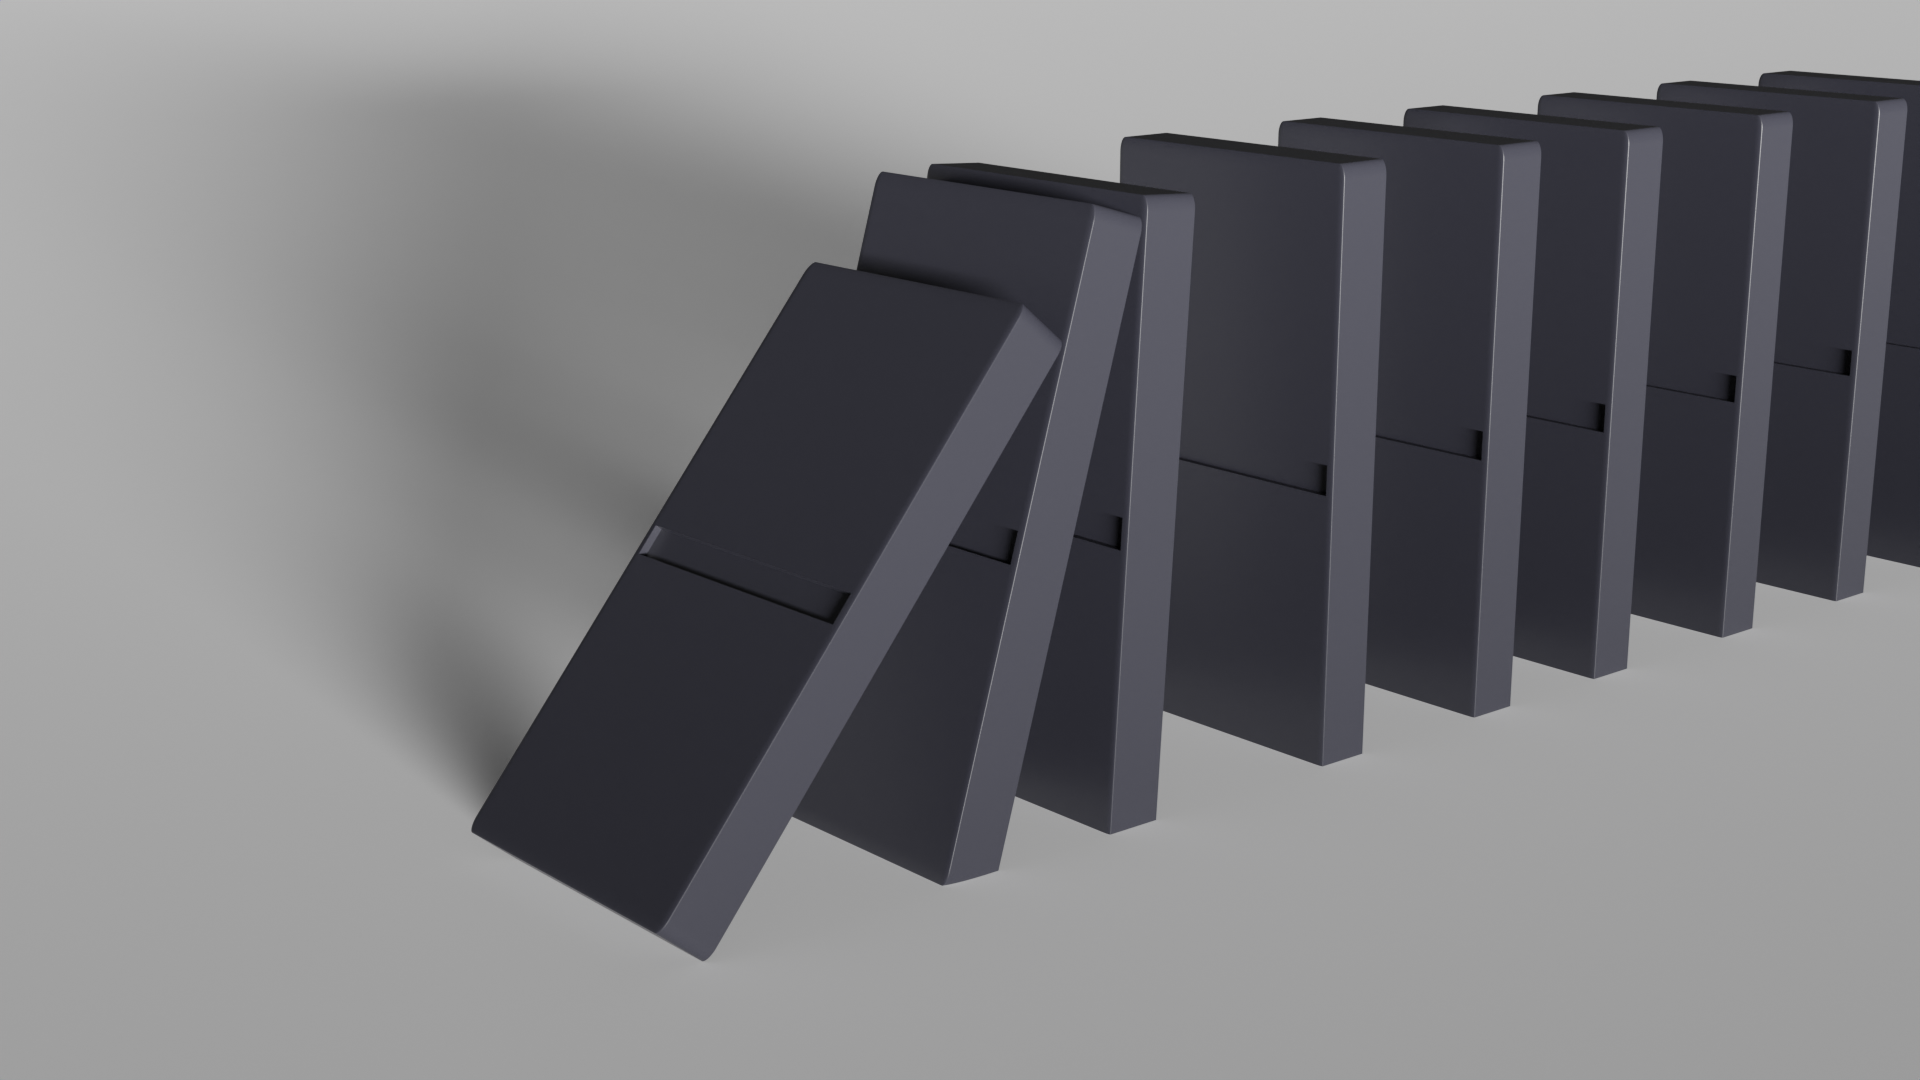
\includegraphics[scale=\fullhd]{ch02_domino_indukce.png}
    \caption{Důkaz indukcí lze přirovnat k~efektu padajícího domina.}
    \label{fig:domino}
\end{figure}
Krok \ref{item:indukcni_krok} se nazývá \emph{indukční krok} a předpoklad, že dokazované tvrzení platí pro nějaké $n=n_0$ se nazývá \emph{indukční předpoklad}. Někdy se v~důkazech indukcí pro upřesnění specifikuje, podle jaké proměnné dané tvrzení dokazujeme. V~tomto případě bychom řekli \emph{"indukcí podle $n$"}. (Inspirováno \cite{MatousekNesetril2009}, str. 32.)\par
Tento postup vychází z~tzv. \emph{principu matematické indukce}, který lze zformulovat jako větu.
\begin{theorem}[Princip matematické indukce]
    Nechť pro každé $n\in\N$ je $\varphi_n$ libovolný výrok. Pokud platí
    \begin{enumerate}[label=(\roman*)]
        \item $\varphi_1$ a
        \item $\forall k\in\N: \varphi_k \implies \varphi_{k+1}$,
    \end{enumerate}
    pak platí $\forall n\in\N: \varphi_n$.
\end{theorem}
(Převzato z~\cite{ChartrandPolimeniZhang2014}, str. 144.)\\
Tuto větu v~různých textech lze najít i v~jiných formulacích. Její důkaz však vyžaduje složitější znalosti. Uveďme si ještě jeden příklad.
\begin{convention}
    Při aplikaci indukčního předpokladu se někdy píše zkratka \emph{I.~P.}, čehož se budeme držet v~dalším textu.
\end{convention}
\begin{proposition}
    Pro každé přirozené $n\geq 5$ platí $2^n>n^2$.
\end{proposition}
\begin{proof}
    Tvrzení dokážeme indukcí podle $n$.
    \begin{itemize}
        \item Pro nejmenší hodnotu $n=5$ dostáváme $2^5=32>5^2=25$, což jistě platí.
        \item Nyní dokážeme indukční krok. Předpokládejme, že tvrzení platí pro libovolné $n_0\geq 5$; ukážeme platnost pro $n_0+1$:
        \begin{equation*}
            2^{n_0+1}=2^{n_0}\cdot 2\stackrel{\text{I. P.}}{>} n_0^2 \cdot 2.
        \end{equation*}
        Pro dokázání tvrzení nyní stačí ukázat, že $2n_0^2 > (n_0+1)^2$.
        \begin{align*}
            2n_0^2 &= n_0^2+n_0^2>n_0^2+5n_0=n_0^2+2n_0+3n_0=n_0^2+2n_0+15\\
            &>n_0^2+2n_0+1=(n_0+1)^2.
        \end{align*}
        Celkově tedy dostáváme $2^{n_0+1}>(n_0+1)^2$.
    \end{itemize}
    Podle principu matematické indukce platí $\forall n\geq 5: 2^n>n^2$, což jsme chtěli dokázat.
\end{proof}
(Převzato z~\cite{ChartrandPolimeniZhang2014}, str. 153.)
% V sekci \ref{sec:mnoziny_a_cisla} o množinách a číslech jsme si slíbili, že si dokážeme tvrzení o mohutnosti potenční množiny libovolné konečné množiny. Existuje více způsobů, jak platnost tohoto tvrzení dokázat (hodně z nich jsou více kombinatorického charakteru). My si jej však dokážeme indukcí pomocí poměrně hezkého triku.
\begin{proposition}
    Nechť $X$ je libovolná $n$-prvková množina. Pak $\sizeof{\powset{X}}=2^n$.
\end{proposition}
\begin{proof}
    Postupujme indukcí podle mohutnosti $n$ množiny $X$. Pro $n=0$ obsahuje potenční množina množiny $X$ pouze prázdnou množinu, tj. $\sizeof{\powset{\emptyset}}=2^0=1$.\par
    Předpokládejme, že tvrzení platí pro množinu o~$n_0$ prvcích. Pro důkaz indukčního kroku mějme množinu $X$ o~$n_0+1$. Vezměme libovolný prvek $x \in X$. Prvky potenční množiny $\powset{X}$ si rozdělíme do množin $T$ a $T^\prime$ takto:
    \begin{itemize}
        \item $T=\set{Q \in \powset{X} \admid x\in Q}$ a
        \item $T^\prime=\set{Q \in \powset{X} \admid x\notin Q}$.
    \end{itemize}
    Tedy v~$T$ se nachází všechny podmnožiny množiny $X$ obsahující prvek $x$ a v~$T^\prime$ všechny podmnožiny, které jej neobsahují. Z~definice lze vidět, že $T$ a $T^\prime$ jsou disjunktní, tj. $T \cap T^\prime=\emptyset$ a tedy $X=T\cup T^\prime$. Jaké jsou mohutnosti $T$ a $T^\prime$? Množina $T^\prime$ obsahuje všechny podmnožiny množiny $X\setminus\set{x}$ a tedy podle indukčního předpokladu má $2^{n_0}$ podmnožin, tj. $\sizeof{\powset{X\setminus\set{x}}}=2^{n_0}$.\par
    Jak vypadají množiny obsažené v~$T$? Uvažme libovolnou podmnožinu $A^\prime$ množiny $X$, která neobsahuje prvek $x$. Taková množina musí být (z~definice) prvkem množiny $T^\prime$. Pokud nyní položíme množinu $A=A^\prime\cup \set{x}$, získáme tak množinu obsahující prvek $x$ a tudíž $A\in T$. Naopak pokud bychom měli množinu $B$ obsahující prvek $x$, tj. $B\in A$, pak definováním $B^\prime=B\setminus \set{x}$ získáme množinu z~$T^\prime$. To však znamená, že každé množině $A^\prime\in T^\prime$ odpovídá právě jedna množina $A\in T$.\par
    Z~toho plyne, že počet množin v~$T$ je stejný\footnote{Formálně vzato jsme sestrojili \emph{bijekci} mezi množinami $T$ a $T^\prime$, kde obrazem množiny $A\in T$ je $A\setminus \set{x}\in T^\prime$. Termín je zaveden v~sekci \ref{sec:zobrazeni}.} jako v~$T^\prime$, tj. $\sizeof{T}=\sizeof{T^\prime}$, což podle již aplikovaného indukčního předpokladu znamená, že $\sizeof{T}=2^{n_0}$. Protože však množiny $T$ a $T^\prime$ jsou disjunktní, pak celkový počet prvků je $2^{n_0}+2^{n_0}=2^{n_0+1}$, což jsme chtěli dokázat.
\end{proof}
\chapter{Dodatky k logice}\label{chap:dodatky_k_logice}
V kapitole o výrokovém a predikátovém počtu jsme pracovali s výrokovými a později predikátovými formulemi, kde jsme si pouze neformálně vysvětlili, co pod těmito termíny rozumíme. Formálněji můžeme k těmto záležitostem přistoupit pomocí následující metadefinice.
\begin{definition}[Výroková a atomická formule]\label{def:vyrokova_a_atomicka_formule}
    $ $\par
    \begin{enumerate}[label=(\roman*)]
        \item\label{item:formule_1} Každá výroková proměnná je \emph{výroková formule} (tzv. \emph{atomická formule}).
        \item\label{item:formule_2} Jsou-li $\varphi$ a $\psi$ výrokové formule, pak $\neg (\varphi)$, $(\varphi) \land (\psi)$, $(\varphi) \lor (\psi)$, $(\varphi) \implies (\psi)$ a $(\varphi) \iff (\psi)$ jsou také výrokové formule.
        \item\label{item:formule_3} Výraz, který nelze získat pomocí pravidel \ref{item:formule_1} a \ref{item:formule_2} není výrokovou formulí.
    \end{enumerate}
\end{definition}
(Převzato z \cite{Fuchs2003}, str. 14 a \cite{BalcarStepanek1986}, str. 30).\par
Definice výrokové formule \ref{def:vyrokova_a_atomicka_formule} nám v podstatě říká, jakým způsobem můžeme sestrojit potenciálně všechny možné formule. Mějme výrokové proměnné $A$, $B$ a $C$. Ty jsou podle \ref{item:formule_1} v definici \ref{def:vyrokova_a_atomicka_formule} výrokovými formulemi. Podle \ref{item:formule_2} jsou pak formulemi i výrazy
\begin{equation}\label{eq:vyrokove_formule_z_definice}
    (A) \land (B)\;,\;(A) \lor (C)\;\text{a}\;\neg(B).
\end{equation}
Nyní můžeme opakovaně použít \ref{item:formule_2} k sestrojení dalších složitějších formulí. Tedy užitím formulí \eqref{eq:vyrokove_formule_z_definice} můžeme dále postupně sestrojit např. výrazy
\begin{equation*}
    \bigl((A) \land (B)\bigr) \implies \bigl((A) \lor (C)\bigr)\quad\text{a}\quad\Bigl((A) \land \bigl(\neg(B)\bigr)\Bigr) \iff \Bigl(\neg\bigl((A) \lor (B)\bigr)\Bigr),
\end{equation*}
které jsou opět podle \ref{item:formule_2} výrokovými formulemi. Opětovným užitím \ref{item:formule_2} pak je dále výrokovou formulí např.
\begin{equation*}
    \Bigl(\bigl((A) \land (B)\bigr) \implies \bigl((A) \lor (C)\bigr)\Bigr) \implies \bigg(\Bigl((A) \land \bigl(\neg(B)\bigr)\Bigr) \iff \Bigl(\neg\bigl((A) \lor (B)\bigr)\Bigr)\bigg).
\end{equation*}
Takto můžeme postupovat dál a opakovanou aplikací pravidla \ref{item:formule_2} vytvořit ještě složitější výrokové formule.\par
Naopak pokud bychom uvážili nějaký výraz, můžeme obdobně zjistit, jestli se jedná o výrokovou formuli či nikoliv.
\begin{example}\label{ex:overeni_formule}
    Mějme výraz
    \begin{equation*}
        \varphi\sim\bigl((A) \land (C)\bigr) \iff \Bigl(\bigl((A) \lor (B)\bigr) \implies \neg(C)\Bigr).
    \end{equation*}
    Ověřte, zda $\varphi$ je výroková formule.\par
    \begin{solution}
        Aby $\varphi$ byla formule, musí být
        \begin{equation*}
            \varphi_1\sim(A) \land (C)\quad\text{a}\quad\varphi_2\sim\bigl((A) \lor (B)\bigr) \implies \neg(C)
        \end{equation*}
        též formulemi. Výraz $\varphi_1$ zřejmě je formulí, neboť $A$ a $C$ jsou atomické formule. Ovšem u $\varphi_2$ lze již vidět, že výraz nesplňuje definici výrokové formule, neboť u $\neg(C)$ chybí vnější závorky. Z bodu \ref{item:formule_3} definice \ref{def:vyrokova_a_atomicka_formule} tedy plyne, že výraz $\varphi$ \textbf{není výrokovou formulí}, neboť jej nelze získat pomocí pravidel \ref{item:formule_1} a \ref{item:formule_2}.
    \end{solution}
\end{example}

Čtenáře možná již napadlo, že formule, které jsme sestrojili z definice \ref{def:vyrokova_a_atomicka_formule}, jsou zapsány poměrně komplikovaně, především co do nadměrného používání závorek. Např. výraz
\begin{equation}\label{eq:poradi_operaci}
    A \land \neg C,
\end{equation}
není podle \ref{def:vyrokova_a_atomicka_formule} výrokovou formulí. I přesto je však nejspíše zřejmé, že tímto zápisem vyjadřujeme výrok "Platí $A$ a zároveň neplatí $C$.". Nebo vrátíme-li se k příkladu \ref{ex:overeni_formule}, i při vypuštění uzávorkování u výrazu $\varphi_2$ by dávalo smysl interpretovat výraz
\begin{equation*}\label{eq:vypusteni_uzavorkovani}
    A \lor B \implies \neg C
\end{equation*}
jako výrok "Jestliže platí $A$ a zároveň $B$, pak neplatí $C$.".
\chapter{Dodatky k axiomům teorie množin}\label{chap:dodatky_k_axiomum_tm}
\section{Důkazy aritmetických vlastností množin}
Ještě jedny známé vztahy pro množiny jsou tzv. \emph{de Morganovy vzorce} (viz obrázek \ref{fig:de_morgan}), které si zde zformulujeme jako větu.
\begin{theorem}[de Morganovy vzorce]
    Nechť $A,X_1,\dots,X_n$ jsou libovolné množiny. Pak platí
    \begin{enumerate}[label=(\roman*)]
        \item\label{item:de_morgan_1} $\displaystyle A \setminus \left(\bigcup\limits_{i=1}^{n}{X_i}\right)=\bigcap\limits_{i=1}^{n}{(A \setminus X_i)}$,
        \item\label{item:de_morgan_2} $\displaystyle A \setminus \left(\bigcap\limits_{i=1}^{n}{X_i}\right)=\bigcup\limits_{i=1}^{n}{(A \setminus X_i)}$.
    \end{enumerate}
\end{theorem}
\begin{proof}
    Nejdříve se zamysleme, co vlastně říkají dané rovnosti. Vyjadřují, že množiny a pravé a levé straně jsou si rovny. Z axiomu extenzionality \ref{item:axiom_extenzionality} víme, že to platí právě tehdy, když mají dané množiny stejné prvky.\par
    Ukážeme pouze platnost \ref{item:de_morgan_1}, avšak důkaz \ref{item:de_morgan_2} je zcela analogický. Budiž dán libovolný prvek $x\in A \setminus \left(\bigcup_{i=1}^{n}{X_i}\right)$. Ukážeme, že $x\in\bigcap_{i=1}^{n}{(A \setminus X_i)}$. Z definice rozdílu množin (viz \ref{def:prunik_rozdil}) tedy musí platit
    \begin{equation*}
        x\in A \setminus \left(\bigcup\limits_{i=1}^{n}{X_i}\right)\iff x\in A \land x\notin \bigcup\limits_{i=1}^{n}{X_i}.
    \end{equation*}
    Protože však $x$ nenáleží sjednocení množin $X_1,\dots,X_n$, pak nenáleží (podle definice \ref{def:sjednoceni}) žádné z nich:
    \begin{equation*}
        x\in\bigcup\limits_{i=1}^{n}{X_i}\iff\forall i\in\set{1,\dots,n}: x\notin X_i.
    \end{equation*}
    Tedy víme, že platí:
    \begin{equation*}
        x\in A \land \forall i\in\set{1,\dots,n}: x\notin X_i.
    \end{equation*}
    Pokud prvek $x$ náleží množině $A$ a zároveň nenáleží žádné z množin $X_1,\dots,X_n$, pak nenáleží ani množině $A\setminus X_i$ pro libovolné $i$, kde $1\leq i\leq n$. Tj.
    \begin{equation*}
        x\in A \land (\forall i\in\set{1,\dots,n}: x\notin X_i)\iff \forall i\in\set{1,\dots,n}: x\in A\setminus X_i.
    \end{equation*}
    Z tohoto faktu již lze vidět, že $x$ nutně leží v průniku těchto množin, tzn.
    \begin{equation*}
        x\in\bigcap\limits_{i=1}^{n}{(A \setminus X_i)},
    \end{equation*} 
    což jsme chtěli dokázat.
\end{proof}
\begin{figure}[H]
	\centering
	\includegraphics[scale=0.7]{ch03_de_Morganovy_vzorce.pdf}
    \caption{De Morganovy vzorce pro $n=2$.}
    \label{fig:de_morgan}
\end{figure}

\section{Schéma axiomů nahrazení}\label{sec:schema_axiomu_nahrazeni}
\begin{align*}
    \forall u\,\forall v\,\forall v^\prime\,(\varphi(u,v) \land \varphi(u,v^\prime) \implies v=v^\prime)\implies\\ \implies \forall a\,\exists z\,\forall x\,\bigl(x\in z \iff \exists y\,(y\in a \land \varphi(y,x))\bigr),
\end{align*}
kde formule $\varphi(u,v)$ neobsahuje proměnné $v^\prime$ a $z$.\par
Tento axiom je pravděpodobně nejsložitější, co do jeho zápisu. Zaměřme se nyní pouze na předpoklad
\begin{equation*}
    \forall u\,\forall v\,\forall v^\prime\,(\varphi(u,v) \land \varphi(u,v^\prime) \implies v=v^\prime).
\end{equation*}
Ten udává, jakou vlastnost musí splňovat formule $\varphi(u,v)$. Tvrzení je takové, že pokud existují množiny $v,v^\prime$ takové, že platí $\varphi(u,v)$ i $\varphi(u,v^\prime)$, pak množiny $v$ a $v^\prime$ musí být stejné. Resp. předpoklad požaduje, aby pro každé $u$ platila formule $\varphi(u,v)$ pro nejvýše jeden prvek $v$. Ekvivalentně bychom toto mohli napsat jako
\begin{equation*}
    \forall u\,\exists! v: \varphi(u,v).
\end{equation*}
Toto by nám již mělo být povědomé. Podobně jsme definovali zobrazení v definici \ref{def:zobrazeni}. V tomto případě můžeme tak $\varphi$ chápat jako formuli udávající, zda obrazem prvku $u$ je prvek $v$.\par
Druhá část
\begin{equation*}
    \forall a\,\exists z\,\forall x\,\bigl(x\in z \iff \exists y\,(y\in a \land \varphi(y,x))\bigr)
\end{equation*}
nám zaručuje, že všechny prvky $v$, kterým odpovídá (v rámci formule $\varphi(u,v)$) nějaký prvek $u\in a$, tvoří množinu $z$. Stručně řečeno, \textbf{obrazem libovolné množiny při definovatelném zobrazení je opět množina}.\par
Tento axiom nebyl součástí původních Zermelových axiomů. Posléze se však ukázalo, že existují množiny, jejichž existence není zbývajícími axiomy implikovaná. Např.
\begin{equation*}
    m=\set{x,\powset{x},\powset{\powset{x}},\powset{\powset{\powset{x}}},\dots},
\end{equation*}
kde $x\neq\emptyset$. Z axiomu nekonečna zaručující existenci nekonečné množiny $z$ víme, že pokud $x$ je prvkem $z$, pak i $x\cup\set{x}$ je prvkem $z$. Není těžké si rozmyslet, že toto pro $m$ není splněno. Nicméně při vhodné volbě formule $\varphi$ lze definovat zobrazení prvků nějaké aktuálně nekonečné množiny postulované axiomem nekonečna na množiny $x,\powset{x},\powset{\powset{x}},\dots$ a podle axiomu nahrazení tak tyto obrazy
\begin{equation*}
    \set{x,\powset{x},\powset{\powset{x}},\powset{\powset{\powset{x}}},\dots}
\end{equation*}
tvoří opět množinu.

\section{Axiom fundovanosti}\label{sec:axiom_fundovanosti}
\begin{equation*}
    \forall a\,\Bigl(a\neq\emptyset \implies \exists x:\bigl(x\in a \land x\cap a=\emptyset\bigr)\Bigr)
\end{equation*}
Tento axiom slouží svým způsobem jako omezení množin, které lze uvažovat. Tvrzení je takové, že každá neprázdná množina musí obsahovat alespoň jeden prvek, který je s ní \emph{disjunktní} (tj. má s ní prázdný průnik). Tím zamezujeme existenci některých typů množin, jako třeba množiny obsahující samy sebe, tj. $a\in a$. Jmenovitě např.
\begin{equation*}
    a=\set{a},\;b=\set{b,\emptyset}\;\text{a jiné.}
\end{equation*}
Lze se snadno přesvědčit, že při existenci takových množin by axiom fundovanosti byl porušen. Pokud bychom připustili např. existenci množiny $x^\prime$, pro kterou by platilo, že $x^\prime\in x^\prime$, pak podle axiomu dvojice \ref{item:axiom_dvojice} je též množinou i $u=\set{x^\prime}$. Podle axiomu fundovanosti musí $u$ obsahovat prvek $x$, takový, že $x\cap x^\prime=\emptyset$. Protože však pouze $x^\prime$ je prvkem $u$, pak musí nutně platit (protože $x^\prime\neq\emptyset$), že $x^\prime\cap u=\emptyset$. To ale neplatí!
\begin{equation*}
    x^\prime\cap\set{x^\prime}=x^\prime,
\end{equation*}
neboť $x^\prime\in x^\prime$. Tzn. $u$ tedy \textbf{nesplňuje} axiom fundovanosti a není tak množinou v \ZF{}.\par
Dalšími důsledky axiomu fundovanosti je vyloučení cyklů v relaci "býti prvkem", tj. např.
\begin{equation*}
    x_1\in x_2\in x_3\in x_1.
\end{equation*}
Trochu obecněji lze nahlédnout, že nikdy tak nemůže nastat situace, kdy bychom našli nekonečný řetězec "do sebe zanořených" množin
\begin{equation*}
    \dots \in x_n\in \dots\in x_2\in x_1\in x_0.
\end{equation*}
\medskip

Axiom fundovanosti tedy slouží jako obecná charakteristika všech myslitelných množin v \ZF{}. Oproti všem ostatním je tedy trochu jiného charakteru, neboť doposud zmíněné axiomy byly spíše "konstrukční". Jejich postupnou aplikací jsme byli schopni sestrojit z menších množin množiny větší. Lze ukázat, že axiom fundovanosti je ekvivalentní s tvrzením, že všechny množiny v \ZF{} lze generovat z prázdné množiny opakovanou aplikací axiomu potence a sumy.
\chapter{Dodatky k~budování číselných množin}\label{chap:dodatky_k_budovani_cis_mn}
\begin{theorem}
    $(\N_0,\leq)$ je lineárně uspořádaná množina.
\end{theorem}
\begin{proof}
    Je-li množina $\N_0$ lineárně uspořádaná vzhledem k~relaci "$\leq$", pak tato relace musí být \textbf{reflexivní}, \textbf{antisymetrická} a~\textbf{tranzitivní} (pro připomenutí viz definice \ref{def:dulezite_vlastnosti_relaci}) a~dále každá dvojice prvků $n,m\in\N_0$ musí být porovnatelná, tj. $n\leq m\lor m\leq n$.
    \begin{itemize}
        \item \textbf{Reflexivita}. Z definice relace "$\leq$" v~\ref{def:nerovnosti} triviálně pro libovolné přirozené číslo $n$ platí $n\leq n$.
        \item \textbf{Antisymetrie}. Nechť $n,m\in\N_0$, přičemž $n\leq m \land m\leq n$. Chceme ukázat, že $n=m$. Pokud platí $n\leq m \land m\leq n$, pak musí platit
        \begin{equation*}
            (n<m\lor n=m) \land (m<n\lor n=m)\;\text{neboli}\;n=m\lor (n<m\land m<n).
        \end{equation*}
        Případ $n<m\land m<n$ nemůže nastat, což lze ukázat sporem: nechť platí $n<m\land m<n$, tj. podle definice $n\in m\land m\in n$. Z bodu \ref{item:vlastnost_2_1} lemmatu \ref{lem:vlastnosti_prirozenych_cisel_2} by plynulo $n\subset m\land m\subset n$ a~z~tranzitivity inkluze máme $n\subset n$, což je spor.
        \item \textbf{Tranzitivita}. Nechť $n,m,\ell\in\N_0$, taková, že platí $n\leq m \land m\leq\ell$. Chceme ukázat, že $n\leq\ell$.\par
        Pokud platí $n=m$, $m=\ell$ nebo $n=\ell$, pak tvrzení jistě platí. Předpokládejme nyní, že $n\neq m\land m\neq\ell\land n\neq\ell$. Podle bodu \ref{item:vlastnost_1_3} lemmatu \ref{lem:vlastnosti_prirozenych_cisel_2} dostáváme $n\subset m\land m\subset\ell$ a~tedy $n\subset\ell$. Opět podle tvrzení \ref{item:vlastnost_1_3} odvodíme $n\leq\ell$.
    \end{itemize}
    Tedy relace "$\leq$" na $\N_0$ je skutečně uspořádáním. Fakt, že toto uspořádání je lineární plyne přímo z důsledku \ref{cor:porovnatelnost}.
\end{proof}
\chapter{Dodatky k~porovnávání nekonečných množin}\label{chap:dodatky_k_porovnavani_nekonecnych_mn}
Dodatečná ukázka Cantorova diagonálního argumentu při důkazu Cantorovy věty pro spočetné množiny.
\begin{theorem}\label{thm:cantorova_veta_spocetne}
    Pro libovolnou spočetnou množinu $X$ platí
    \begin{equation*}
        X\prec\powset{X}.
    \end{equation*}
\end{theorem}
\begin{proof}
    Ukážeme, že $X\napprox\powset{X}$ (případ $X\preccurlyeq\powset{X}$ již známe). K tomu lze přistoupit sporem. Pro spor nechť $X\approx\powset{X}$, tzn. existuje bijektivní zobrazení $\map{f}{X}{\powset{X}}$. Obdobně jako v~důkazu věty \ref{thm:N_a_R}, i zde ukážeme, že $f$ není surjektivní. Obrazy prvků $x_i\in X$ tak můžeme "uspořádat" do "seznamu" $f(x_1),f(x_2),f(x_3),\dots$. Podmnožinu $A$ můžeme z množiny sestrojit $X$ tak, že pro každý z prvků množiny $X$ určíme, zda náleží $A$ či nikoliv. Označíme-li si případ $x\in A$ písmenem A a případ $x\notin A$ jako N, pak zmíněný "seznam" bychom mohli znázornit podobně jako na obrázku \ref{fig:seznam_podmnoziny}.
    \begin{figure}[H]
        \centering
        \includegraphics[scale=\normalipe]{ch06_seznam_podmnoziny.pdf}
        \caption{Podmnožiny (obrazy) množiny $X$ určené náležením každého z prvků.}
        \label{fig:seznam_podmnoziny}
    \end{figure}
    Opět se zaměříme na diagonálu tohoto seznamu.
    \begin{figure}[H]
        \centering
        \includegraphics[scale=\normalipe]{ch06_diagonala_podmnoziny.pdf}
        \caption{Diagonála seznamu podmnožin množiny $X$.}
        \label{fig:diagonala_podmnoziny}
    \end{figure}
    Zkonstruujeme množinu $S$ tak, že každý prvek $x$ na diagonále jí náleží právě tehdy, když nenáleží podmnožině (tedy obrazu $f(x)$) v příslušném řádku. Evidentně množina $S$ je podmnožinou $X$. Zároveň se však od každé podmnožiny na seznamu liší minimálně v prvku na diagonále. To znamená, že $S$ nemůže být na seznamu, čímž dostáváme spor.
\end{proof}
\section{Relace ekvivalence}\label{sec:relace_ekvivalence}
Zmíněné druhy relací nám dovolují definovat dva jejich nejdůležitější typy, jednomu z nichž se budeme dále přednostně věnovat. Začneme prvním z nich.
\begin{definition}[Relace ekvivalence]\label{def:relace_ekvivalence}
    Nechť $R$ je relace na množině $X$. Řekneme, že $R$ je \emph{relací ekvivalence na $X$} (nebo jen \emph{ekvivalencí na $X$}), pokud je \emph{reflexivní}, \emph{symetrická} a \emph{tranzitivní}.
\end{definition}
Ač se to nemusí zdát, tento typ relace má velmi příjemné vlastnosti. Jak si ji představit? Příkladem může být třeba relace $R$ na množině $X=\set{x_1,\dots,x_7}$ znázorněná na obrázku \ref{fig:priklad_relace_ekvivalence} níže.
\begin{figure}[H]
    \centering
    \includegraphics[scale=\normalipe]{ch02_relace_ekvivalence.pdf}
    \caption{Relace ekvivalence $R$ na $X$.}
    \label{fig:priklad_relace_ekvivalence}
\end{figure}
Pokud by však byl např. prvek $x_3$ v relaci prvkem $x_4$, pak by již $R$ nebyla ekvivalencí, jak lze naopak vidět z obrázku \ref{fig:priklad_relace_neekvivalence}.
\begin{figure}[H]
    \centering
    \includegraphics[scale=\normalipe]{ch02_relace_neekvivalence.pdf}
    \caption{Relace $R \cup (x_3,x_4)$ na $X$.}
    \label{fig:priklad_relace_neekvivalence}
\end{figure}
Všimněte si, že na obrázku \ref{fig:priklad_relace_ekvivalence} jsou prvky rozděleny na "ostrůvky", kde v~rámci každého z nich jsou spolu všechny prvky v~relaci\footnote{U relace ekvivalence též říkáme, že prvky jsou spolu \emph{ekvivalentní}.}. (Zkuste si z definice rozmyslet, že to tak vždy musí být.) Zakreslovat relaci ekvivalence dosavadním se tak stává již celkem nevýhodným, neboť pro větší množství ekvivalentních prvků již zakreslovat všechny vztahy šipkami je v~tomto případě poměrně zdlouhavý proces (např. pro 5 ekvivalentních prvků bychom museli kreslit 25 šipek). Úspornější a taktéž názornější pro nás bude si pouze schématicky rozdělit prvky do skupinek (relace mezi nimi z definice ekvivalence považujeme za samozřejmé), např. jako na obrázku \ref{fig:relace_ekvivalence_tridy}.
\begin{figure}[H]
    \centering
    \includegraphics[scale=\normalipe]{ch02_relace_ekvivalence_tridy.pdf}
    \caption{Schématické znázornění ekvivalence $R$ na $X$.}
    \label{fig:relace_ekvivalence_tridy}
\end{figure}
Definujme si nyní tyto "ostrůvky" trochu formálněji.
\begin{definition}[Třída ekvivalence]
    Nechť $R$ je relace ekvivalence na množině $X$ a nechť $x\in X$. Pak definujeme množinu
    \begin{equation*}
        [x]_R=\set{y \admid xRy},
    \end{equation*}
    kterou nazýváme \emph{třída ekvivalence $R$ určená prvkem $x$}.
\end{definition}
Třída ekvivalence $[x]_R$ jistého prvku $x$ tak obsahuje všechny prvky, které jsou s $x$ ekvivalentní. Z příkladu výše je vidět že platí:
\begin{itemize}
    \item $[x_1]_R=[x_2]_R=[x_3]_R=\set{x_1,x_2,x_3}$,
    \item $[x_4]_R=[x_5]_R=\set{x_4,x_5}$,
    \item $[x_6]_R=[x_7]_R=[x_8]_R=\set{x_6,x_7,x_8}$.
\end{itemize}
\begin{example}
    Další příklady relací ekvivalence a jejich tříd.
    \begin{enumerate}[label=(\roman*)]
        \item $(\N,=)$ (rovnost přirozených čísel) je relace ekvivalence, kde každý prvek tvoří samostatnou třídu ekvivalence.
        \begin{align*}
            [1]_R&=\set{1}\\
            [2]_R&=\set{2}\\
            &\vdots
        \end{align*}
        \item Relace \emph{"mít stejnou paritu"}\footnote{Tzn. obě čísla jsou sudá nebo lichá.} na množině $\Z$ je relace ekvivalence o dvou třídách (sudá a lichá čísla).
        \begin{align*}
            [1]_R&=\set{-1,1,-3,3,-5,5,\dots}\\
            [2]_R&=\set{0,-2,2,-4,4\dots}\\
            &\vdots
        \end{align*}
        \item Relace "mít stejný zbytek po celočíselném dělení 5" na množině $\Z$ je relace ekvivalence o pěti třídách (čísla 0--4 jako zbytek po celočíselném dělení).
        \begin{align*}
            [0]_R&=\set{0,5,10,\dots}\\
            [1]_R&=\set{1,6,11,\dots}\\
            [2]_R&=\set{2,7,12,\dots}\\
            [3]_R&=\set{3,8,13,\dots}\\
            [4]_R&=\set{4,9,14,\dots}
        \end{align*}
        \item Relace "mít stejnou absolutní hodnotu" na množině $\R$ je relace ekvivalence, kde každá třída obsahuje prvek $x$ a $-x$ pro všechna $x\in\R$.
        \begin{align*}
            [0]_R&=\set{0}\\
            [1]_R&=\set{-1,1}\\
            [\sqrt{2}]_R&=\set{\sqrt{2},-\sqrt{2}}\\
            [\sqrt[4]{30}]_R&=\set{\sqrt[4]{30},-\sqrt[4]{30}}\\
            &\vdots
        \end{align*}
    \end{enumerate}
\end{example}

\section{Mohutnost množiny}\label{sec:mohutnost_mnoziny}
V sekci jsme v~definici subvalence a ekvipotence \ref{def:subvalence_a_ekvipotence} zmínili pojem "mohutnost" (ostatně zmínili jsme jej ue v~distorickém úvodu). Již víme, co je míněno pod tvrzením, že množina "má větší/stejnou mohutnost" jako jiná množina. To nám však pouze dává představu, jak mohutnosti porovnávat. Jak tuto vlastnost množiny explicitně vyjádřit?\par
V případě konečných množin rozumíme pod "mohutností" množiny jednoduše její velikost (tj. počet prvků), kterou reprezentuje nějaké přirozené číslo. U nekonečných množin je to však složitější. Nelze říci, že mohutnost je $\infty$. Podle této logiky by pak muselo platit např. $\sizeof{\N}=\sizeof{\R}=\infty$. To by však nebylo konzistentní s definicí, že dvě množiny mají stejnou mohutnost, když mezi nimi existuje bijekce, protože podle věty \ref{thm:N_a_R} víme, že $\R\preccurlyeq\N$. Na mohutnost množiny lze nahlížet i trochu abstraktněji.
\medskip

Pro lehčí pochopení se na chvíli přesuňme ke geometrii. Uvážíme-li relaci "být rovnoběžný s", tj. "$\parallel$" na množině všech přímek v~rovině, jaké vlastnosti splňuje?
\begin{itemize}
    \item \textbf{Reflexivita}. Každá přímka je rovnoběžná sama se sebou, tj. pro přímku $p$ platí $p\parallel p$.
    \item \textbf{Symetrie}. Platí-li $p\parallel q$, pak platí i $q\parallel p$.
    \item \textbf{Tranzitivita}. Je-li přímka $p$ rovnoběžná s přímkou $q$ a zároveň $q$ je rovnoběžná s přímkou $r$, pak určitě $p\parallel r$.
\end{itemize}
Tedy "$\parallel$" je relací ekvivalence. Na základě tohoto poznatku, máme-li libovolnou přímku $p$, jaké přímky obsahuje třída ekvivalence $[p]_\parallel$? Budou to právě takové přímky, které jsou rovnoběžné s přímkou $p$. Jak bychom definovali \emph{směr} přímky? Zkuste se zamyslet, než budete pokračovat.\par
Zkusme se ale zpětně zaměřit na třídy ekvivalence "$\parallel$". Uvážíme-li libovolnou z nich, pak přímky jí náležící mají vždy shodný směr. To znamená, že výběrem kterékoliv třídy ekvivalence je směr jednoznačně určen podle náležících přímek. Tedy celkově: za směr přímky $p$ prohlásíme třídu ekvivalence $[p]_\parallel$.
\medskip

Tato úvaha nám zde velmi pomůže. Ačkoliv sice netušíme, co je to mohutnost množiny, přesto dokážeme určit (v principu), zda libovolné množiny $X$ a $Y$ mají stejnou mohutnost, nebo nemají.
\begin{lemma}
    Ekvipotence $\approx$ je relací ekvivalence\footnote{Zde se jedná o tzv. \emph{třídovou relaci} na tzv. \emph{univerzální třídě} (často označované $\mathbb{V}$), tedy "souhrnu" všech množin. Tento "souhrn" nemůže být množinou, neboť bychom tak došli ke sporu v \ZF{}. Třídy představují v teorii množin "nadstavbu" termínu množina. Obecně platí, že každá množina je třída, ale ne každá třída je množina. Pro hlubší pochopení doporučuji knihu \cite{BalcarStepanek1986}, str. 45--50}.
\end{lemma}
\begin{proof}
    Z definice relace ekvivalence stačí ověřit, že $\approx$ je reflexivní, symetrická a tranzitivní. Mějme libovolné množiny $X,Y,Z$.
    \begin{itemize}
        \item \textbf{Reflexivita}. Jistě platí $X\approx X$. Za bijektivní zobrazení stačí zvolit identitu $1_X$.
        \item \textbf{Symetrie}. Pokud $X\approx Y$, pak existuje bijekce $\map{f}{X}{Y}$. Protože $f$ je bijekce, existuje inverzní zobrazení $\map{f^{-1}}{Y}{X}$, které je též bijekcí. Tzn. platí i $Y\approx X$.
        \item \textbf{Tranzitivita}. Nechť $X\approx Y$ a zároveň $Y\approx Z$. Pišme $\map{f}{X}{Y}$ a $\map{g}{Y}{Z}$. Definujme zobrazení $h=g\circ f$. Podle tvrzení \ref{prop:vlastnosti_skladani_zobrazeni} je $\map{h}{X}{Z}$ bijekce a tedy $X\approx Z$.
    \end{itemize}
    Tedy $\approx$ je relací ekvivalence.
\end{proof}
Pro libovolnou množinu $X$ tak třída ekvivalence $[X]_\approx$ obsahuje všechny množiny, které mají stejnou mohutnost jako $X$. Tzn.
\begin{equation*}
    \forall Y\in [X]_\approx: Y\approx X.
\end{equation*}
Víme tak, že každá z množin v~libovolné třídě ekvivalence má stejnou mohutnost. Tuto třídu bychom pak mohli prohlásit za její mohutnost. V případě konečných množin, kde za mohutnost považujeme přirozené číslo, se jedná o alternativní pohled.\par
Mohutnosti představují v teorii množin tzv. \emph{kardinální čísla}, která lze definovat způsobem popsaným výše. Jedná se tak o zobecnění myšlenky počtu prvků u konečných množin. Podobně jako na přirozených číslech, i na kardinálních číslech lze definovat smysluplnou aritmetiku.

\openright
\end{document}
